\section{Asymmetry}
\label{sec:asymmetry}

Under partner symmetry the common and zero-sum subspaces are eigenspaces of the adjustment matrix (\cref{prop:decomposition}), so average protection moves the effective exchange rate and relative treatment moves bilateral rates around it. Asymmetry in country sizes, origin weights or home bias breaks this structure. This section asks which of the symmetric results survive. Two weighted averages of bilateral responses must be kept apart: the trade-weighted NEER of \cref{sec:decomposition}, with weights $w_{Aj}$ that combine $A$'s imports from and exports to $j$, and the aggregate terms of trade, which weight the same responses by $A$'s import shares $b_{Aj}$. The two coincide at the symmetric benchmark and differ away from it, and the second is the welfare-relevant object.

\subsection{The aggregate terms of trade and welfare}
\label{sec:welfare}

Let $b_{Aj}$ denote partner $j$'s share in $A$'s baseline import expenditure, so that $\sum_{j\neq A}b_{Aj}=1$, and let $R^B_j\equiv\partial\nu_j/\partial\tau_{AB}$ be the response of $A$'s bilateral rate against $j$ to a marginal tariff by $A$ on $B$; $R^B_j>0$ is a depreciation of $A$ against $j$. Define
\begin{equation}
R_{A|B}\equiv\sum_{j\neq A}b_{Aj}R^B_j.
\label{eq:RAB}
\end{equation}
Since each producer's price is fixed in its own currency, the log change in $A$'s import-weighted aggregate terms of trade is $-\sum_{j\neq A}b_{Aj}\,d\nu_j$, and a marginal tariff on $B$ improves it if and only if $R_{A|B}<0$.

The welfare result is stated at a balanced free-trade baseline of the model of \cref{sec:model} with interior shares, lump-sum rebate of tariff revenue, and exchange rates differentiable in tariffs, which holds whenever $J$ is nonsingular.

\begin{lemma}[First-order welfare]
\label{lem:welfare}
Under these assumptions, let $d\tau$ be any marginal tariff vector, imposed by $A$ or by other countries. To first order, the change in the welfare of $A$'s representative household, in units of $A$'s income, is
\begin{equation}
\frac{dU_A}{U_A'\,I_A}=-\,m_A\sum_{j\neq A}b_{Aj}\,d\nu_j,
\label{eq:welfare}
\end{equation}
where $m_A$ is $A$'s import share of income. A marginal tariff change therefore raises $A$'s own welfare to first order if and only if it improves $A$'s import-weighted aggregate terms of trade.
\end{lemma}

\noindent At free trade, the first-order tariff-revenue gain offsets the direct increase in import prices, leaving the welfare effect of the induced exchange-rate adjustment. The formal proof is in \cref{app:proofs}.

Because the first-order welfare effect is linear in the tariff vector, write, for tariffs imposed by $A$,
\begin{equation}
\frac{dU_A}{U_A'\,I_A}=\sum_{j\neq A}g_j\,d\tau_{Aj},\qquad g_j\equiv-m_A\,R_{A|j},
\label{eq:gradient}
\end{equation}
where $R_{A|j}$ is the response \cref{eq:RAB} to a tariff on $j$ alone. The component $g_j$ is the first-order welfare gain to $A$ from a marginal tariff on $j$, and a marginal uniform tariff, $d\tau_{Aj}=dt$ for all $j\neq A$, is worth $\sum_jg_j\,dt$.

\begin{proposition}[Uniform tariffs]
\label{prop:uniform}
Consider any balanced free-trade baseline at which MML and the assumptions of \cref{lem:welfare} hold; country sizes, origin shares, home biases and parameters may differ across countries. Let $A$ impose a marginal uniform tariff on all foreign partners, $d\tau_{Aj}=dt>0$ for all $j\neq A$, with all other tariffs unchanged. Then:
\begin{enumerate}[label=(\roman*)]
\item the tariff disturbs every partner's trade balance by
\begin{equation}
F_j=-f_{Aj}\,\rho_D^A\,dt,\qquad \rho_D^A\equiv\eta_Ah_A+(1-h_A)(1-\alpha_T^A)>0,
\label{eq:uniformF}
\end{equation}
where $h_A$ is $A$'s home share of tradable spending and $\eta_A$, $\alpha_T^A$ are $A$'s own parameters;
\item $A$'s currency appreciates weakly against every partner, $d\nu_j\leq0$, and strictly against every partner if $A$ imports from all of them or $J$ is irreducible;
\item $A$'s import-weighted aggregate terms of trade improve and $A$'s own welfare rises to first order: $\sum_{j\neq A}g_j>0$.
\end{enumerate}
\end{proposition}

\noindent A uniform tariff leaves relative import prices across foreign suppliers unchanged, so cross-origin substitution creates no differential incidence across partners, and the exchange-rate adjustment preserves the conventional aggregate result. The result is local, concerns $A$'s own welfare at a balanced free-trade baseline, and establishes nothing about finite tariffs, retaliation, global welfare, or a globally optimal tariff. It is a local, own-country counterpart of the classical terms-of-trade argument for a small tariff \citep{johnson1953,broda2008,costinot2015}; as in \citet{bagwell1999,bagwell2002}, nondiscrimination confines a country's tariffs to a single terms-of-trade channel. The proof is in \cref{app:proofs}.

A uniform tariff restricts the sum of the partner-specific welfare gradients, not every component separately; a tariff on one partner can therefore still lower $A$'s welfare. With $N=3$, $g_B+g_C>0$, so $g_B<0$ implies $g_C>0$.

\subsection{The aggregate terms-of-trade condition}
\label{sec:totcondition}

Separate the target from the remaining suppliers. Define
\begin{equation*}
\bar R^B_{-B}\equiv\frac{\sum_{j\neq A,B}b_{Aj}R^B_j}{1-b_{AB}},
\end{equation*}
the import-weighted average response of $A$'s rates against all bystanders, each bystander weighted by its share in $A$'s imports from suppliers other than $B$. Then $R_{A|B}=b_{AB}R^B_B+(1-b_{AB})\bar R^B_{-B}$: $A$'s exposure to the target, its import weight on $B$ times the move against $B$, plus its exposure to the bystanders.

\begin{definition}[Aggregate terms-of-trade condition]
\label{def:tot}
Unilateral tariffs by $A$ have the conventional aggregate terms-of-trade effect if, for every target $B$,
\begin{equation}
b_{AB}R^B_B+(1-b_{AB})\bar R^B_{-B}<0.
\label{eq:totcondition}
\end{equation}
\end{definition}

Suppose $A$ appreciates against the target, $R^B_B<0$, and depreciates on average against the bystanders, $\bar R^B_{-B}>0$. The condition then fails if and only if
\begin{equation}
\frac{\bar R^B_{-B}}{-R^B_B}>\frac{b_{AB}}{1-b_{AB}}.
\label{eq:totfail}
\end{equation}
The left side is the \emph{equilibrium incidence}: the average adverse move against bystanders per unit of favorable move against the target. The right side is \emph{relative import exposure}: $A$'s import expenditure on the target relative to its import expenditure on all other suppliers. Both are positive pure numbers. Given $R^B_B<0$, a bilateral reversal against at least one bystander is necessary but not sufficient for an aggregate reversal: the adverse moves must also be large enough and carry enough weight in $A$'s import basket.

In terms of \cref{eq:gradient}, the condition requires every partner-specific component $g_B$ to be positive, whereas \cref{prop:uniform} restricts only their sum. The condition has a three-country algebraic form for any configuration of bystanders, because $\bar R^B_{-B}$ is defined as their import-weighted average; this does not make a heterogeneous bloc a literal representative country (\cref{sec:heterogeneous}).

\subsection{Asymmetric partners in the three-country model}
\label{sec:threecountry}

Fix a balanced free-trade baseline of the three-country model, that is, the import-origin shares $b_{ij}$, the home shares $h_i$, the incomes $y_i$ and all parameters other than $\rho$, and let only $\rho$ vary. Write the local system as $A(\rho)R=F(\rho)$, with $A\equiv-J$ and $R=(R^B_B,R^B_C)'$. Since $\rho$ enters the linearized share responses (\cref{eq:linear}) only through the factor $(1-\rho)$, every entry of $A$ and $F$ is affine in $\rho$, and so is the adjugate of the $2\times2$ matrix $A$. Hence
\begin{equation}
R_{A|B}(\rho)=\frac{b'\adj(A(\rho))F(\rho)}{\det A(\rho)},\qquad
b'\adj(A(\rho))F(\rho)=q_2\rho^2+q_1\rho+q_0\equiv Q_{A|B}(\rho).
\label{eq:Q}
\end{equation}
Under MML $\det A(\rho)>0$, so at every $\rho$ at which MML holds at the fixed baseline, $R_{A|B}$ has the sign of $Q_{A|B}(\rho)$ and the aggregate condition is $Q_{A|B}(\rho)<0$. The bilateral bystander response has the same structure; with a common $\alpha_T$, its numerator has leading coefficient $\alpha_T^2\,b_{AB}b_{AC}b_{CA}b_{CB}(1-h_A)(1-h_C)y_Ay_C>0$ (\cref{app:asym-primitives}).

\begin{proposition}[Three cases]
\label{prop:threecases}
Fix a balanced free-trade baseline of the three-country model as above, and consider values $\rho>0$ at which MML holds at that baseline. The following three cases are those used in this paper; they are not an exhaustive classification of the signs of $(q_2,q_1,q_0)$.
\begin{enumerate}[label=(\alph*)]
\item Symmetric benchmark: $q_2=0$ and $Q_{A|B}(\rho)<0$ for all $\rho$. The aggregate condition always holds.
\item $q_2>0$ and $q_0<0$: $Q_{A|B}$ has exactly one positive root $\rho^*$. The condition holds for $\rho<\rho^*$ and fails for $\rho>\rho^*$.
\item $q_2<0$, $q_1>0$, $q_0<0$ and a positive discriminant: $Q_{A|B}$ has two positive roots $\rho_1<\rho_2$. The condition fails only for $\rho_1<\rho<\rho_2$.
\end{enumerate}
\end{proposition}

Case (b) is the economically central asymmetric case: the conventional aggregate effect holds at low cross-origin substitutability and is reversed above a single threshold. Case (c) requires richer network asymmetry and is reported as a robustness example. The three panels of \cref{fig:tot} are parameterized examples of the three cases (\cref{app:asym-tot}).

\begin{figure}[t]
\centering
\begin{subfigure}[t]{0.32\textwidth}\centering
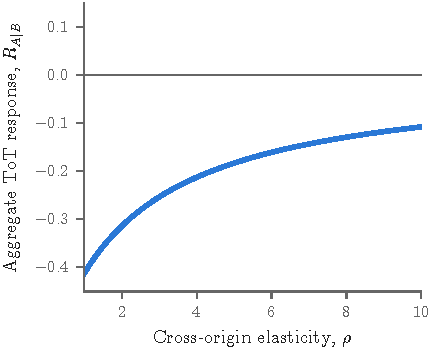
\includegraphics[width=\textwidth]{fig6a_aggregate_tot.pdf}
\caption{Symmetric benchmark}
\end{subfigure}\hfill
\begin{subfigure}[t]{0.32\textwidth}\centering
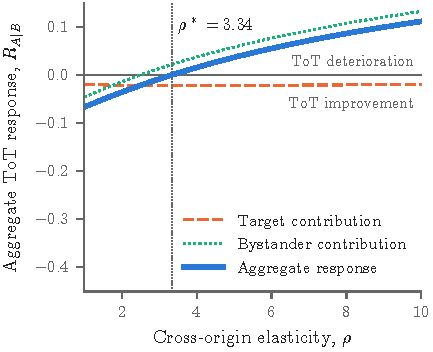
\includegraphics[width=\textwidth]{fig6b_aggregate_tot.pdf}
\caption{Small, low-weight target}
\end{subfigure}\hfill
\begin{subfigure}[t]{0.32\textwidth}\centering
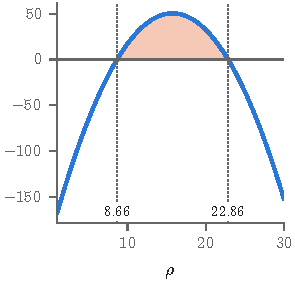
\includegraphics[width=\textwidth]{fig6c_aggregate_tot.pdf}
\caption{Asymmetric network}
\end{subfigure}
\caption{Aggregate terms-of-trade effects under asymmetry. Examples with no reversal, one threshold, and two thresholds. Shading denotes regions in which a marginal discriminatory tariff worsens the aggregate terms of trade.}
\label{fig:tot}
\end{figure}

Aggregate terms-of-trade reversal is more likely when the targeted partner is small relative to untariffed suppliers, when it has a low weight in $A$'s imports, and when foreign suppliers are sufficiently close substitutes. The appreciation against a small or lightly weighted target receives little weight in $A$'s import price index, the adverse movements against larger bystanders receive more, and strong cross-origin substitution redirects expenditure toward those bystanders. In the local model, at a balanced free-trade baseline satisfying MML, a discriminatory marginal tariff can therefore reduce $A$'s own welfare to first order, whereas by \cref{prop:uniform} a marginal uniform tariff at the same baseline raises it. \Cref{app:asym-tot} reports the numerical examples.

\subsection{Effective exchange rates and heterogeneous bystanders}
\label{sec:neer}
\label{sec:heterogeneous}

The NEER uses trade weights $w_{Aj}$, which include $A$'s exports to $j$, whereas the aggregate terms of trade use import weights $b_{Aj}$. Under asymmetry the two weighting schemes differ, so the NEER threshold can differ from the aggregate terms-of-trade threshold; when the target buys much more from $A$ than $A$ buys from it, the favorable move against the target counts for more in the NEER. \Cref{app:asym-tot} reports a numerical illustration.

For $N\geq4$, heterogeneous bystanders generally cannot be collapsed into the exact representative bystander of \cref{prop:composite}. The bloc's average response depends on its internal adjustment structure, including the block $J_{RR}$ of bystanders' responses to their own rates, their responses $J_{RB}$ to the rate against the target, and their disturbances $F_R$ (\cref{app:asym-primitives}), even though the identity $R_{A|B}=b_{AB}R^B_B+(1-b_{AB})\bar R^B_{-B}$ always holds. The three-country structure is therefore a diagnostic of sign mechanisms rather than a quantitative representation of a heterogeneous network.
